\subsection{Implementacja dwupętlowego regulatora PID}
\label{lab:zad3}


%\begin{figure}[H] 
%    \centering
%    % This file was created by matlab2tikz.
%
\definecolor{mycolor1}{rgb}{0.00000,0.44700,0.74100}%
%
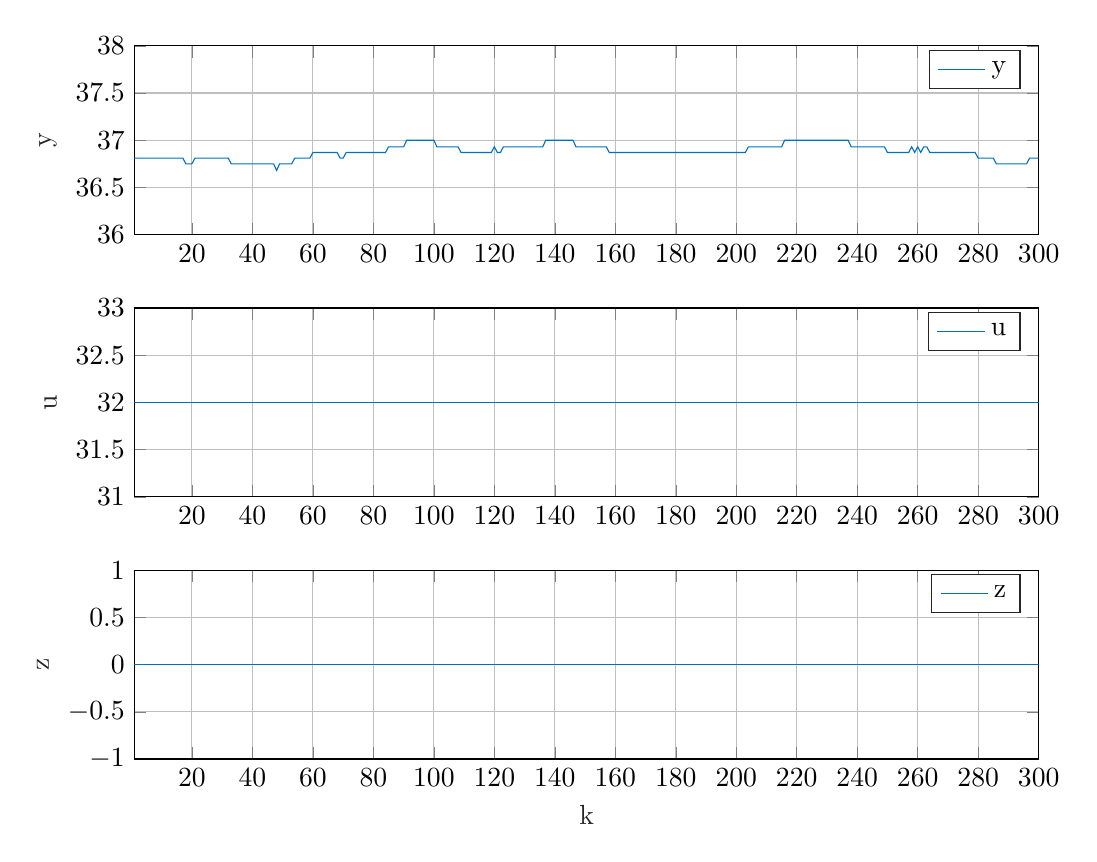
\begin{tikzpicture}

\begin{axis}[%
width=4.521in,
height=0.944in,
at={(0.758in,3.103in)},
scale only axis,
xmin=1,
xmax=300,
ymin=36,
ymax=38,
ylabel style={font=\color{white!15!black}},
ylabel={y},
axis background/.style={fill=white},
xmajorgrids,
ymajorgrids,
legend style={legend cell align=left, align=left, draw=white!15!black}
]
\addplot [color=mycolor1]
  table[row sep=crcr]{%
1	36.81\\
2	36.81\\
3	36.81\\
4	36.81\\
5	36.81\\
6	36.81\\
7	36.81\\
8	36.81\\
9	36.81\\
10	36.81\\
11	36.81\\
12	36.81\\
13	36.81\\
14	36.81\\
15	36.81\\
16	36.81\\
17	36.81\\
18	36.75\\
19	36.75\\
20	36.75\\
21	36.81\\
22	36.81\\
23	36.81\\
24	36.81\\
25	36.81\\
26	36.81\\
27	36.81\\
28	36.81\\
29	36.81\\
30	36.81\\
31	36.81\\
32	36.81\\
33	36.75\\
34	36.75\\
35	36.75\\
36	36.75\\
37	36.75\\
38	36.75\\
39	36.75\\
40	36.75\\
41	36.75\\
42	36.75\\
43	36.75\\
44	36.75\\
45	36.75\\
46	36.75\\
47	36.75\\
48	36.68\\
49	36.75\\
50	36.75\\
51	36.75\\
52	36.75\\
53	36.75\\
54	36.81\\
55	36.81\\
56	36.81\\
57	36.81\\
58	36.81\\
59	36.81\\
60	36.87\\
61	36.87\\
62	36.87\\
63	36.87\\
64	36.87\\
65	36.87\\
66	36.87\\
67	36.87\\
68	36.87\\
69	36.81\\
70	36.81\\
71	36.87\\
72	36.87\\
73	36.87\\
74	36.87\\
75	36.87\\
76	36.87\\
77	36.87\\
78	36.87\\
79	36.87\\
80	36.87\\
81	36.87\\
82	36.87\\
83	36.87\\
84	36.87\\
85	36.93\\
86	36.93\\
87	36.93\\
88	36.93\\
89	36.93\\
90	36.93\\
91	37\\
92	37\\
93	37\\
94	37\\
95	37\\
96	37\\
97	37\\
98	37\\
99	37\\
100	37\\
101	36.93\\
102	36.93\\
103	36.93\\
104	36.93\\
105	36.93\\
106	36.93\\
107	36.93\\
108	36.93\\
109	36.87\\
110	36.87\\
111	36.87\\
112	36.87\\
113	36.87\\
114	36.87\\
115	36.87\\
116	36.87\\
117	36.87\\
118	36.87\\
119	36.87\\
120	36.93\\
121	36.87\\
122	36.87\\
123	36.93\\
124	36.93\\
125	36.93\\
126	36.93\\
127	36.93\\
128	36.93\\
129	36.93\\
130	36.93\\
131	36.93\\
132	36.93\\
133	36.93\\
134	36.93\\
135	36.93\\
136	36.93\\
137	37\\
138	37\\
139	37\\
140	37\\
141	37\\
142	37\\
143	37\\
144	37\\
145	37\\
146	37\\
147	36.93\\
148	36.93\\
149	36.93\\
150	36.93\\
151	36.93\\
152	36.93\\
153	36.93\\
154	36.93\\
155	36.93\\
156	36.93\\
157	36.93\\
158	36.87\\
159	36.87\\
160	36.87\\
161	36.87\\
162	36.87\\
163	36.87\\
164	36.87\\
165	36.87\\
166	36.87\\
167	36.87\\
168	36.87\\
169	36.87\\
170	36.87\\
171	36.87\\
172	36.87\\
173	36.87\\
174	36.87\\
175	36.87\\
176	36.87\\
177	36.87\\
178	36.87\\
179	36.87\\
180	36.87\\
181	36.87\\
182	36.87\\
183	36.87\\
184	36.87\\
185	36.87\\
186	36.87\\
187	36.87\\
188	36.87\\
189	36.87\\
190	36.87\\
191	36.87\\
192	36.87\\
193	36.87\\
194	36.87\\
195	36.87\\
196	36.87\\
197	36.87\\
198	36.87\\
199	36.87\\
200	36.87\\
201	36.87\\
202	36.87\\
203	36.87\\
204	36.93\\
205	36.93\\
206	36.93\\
207	36.93\\
208	36.93\\
209	36.93\\
210	36.93\\
211	36.93\\
212	36.93\\
213	36.93\\
214	36.93\\
215	36.93\\
216	37\\
217	37\\
218	37\\
219	37\\
220	37\\
221	37\\
222	37\\
223	37\\
224	37\\
225	37\\
226	37\\
227	37\\
228	37\\
229	37\\
230	37\\
231	37\\
232	37\\
233	37\\
234	37\\
235	37\\
236	37\\
237	37\\
238	36.93\\
239	36.93\\
240	36.93\\
241	36.93\\
242	36.93\\
243	36.93\\
244	36.93\\
245	36.93\\
246	36.93\\
247	36.93\\
248	36.93\\
249	36.93\\
250	36.87\\
251	36.87\\
252	36.87\\
253	36.87\\
254	36.87\\
255	36.87\\
256	36.87\\
257	36.87\\
258	36.93\\
259	36.87\\
260	36.93\\
261	36.87\\
262	36.93\\
263	36.93\\
264	36.87\\
265	36.87\\
266	36.87\\
267	36.87\\
268	36.87\\
269	36.87\\
270	36.87\\
271	36.87\\
272	36.87\\
273	36.87\\
274	36.87\\
275	36.87\\
276	36.87\\
277	36.87\\
278	36.87\\
279	36.87\\
280	36.81\\
281	36.81\\
282	36.81\\
283	36.81\\
284	36.81\\
285	36.81\\
286	36.75\\
287	36.75\\
288	36.75\\
289	36.75\\
290	36.75\\
291	36.75\\
292	36.75\\
293	36.75\\
294	36.75\\
295	36.75\\
296	36.75\\
297	36.81\\
298	36.81\\
299	36.81\\
300	36.81\\
};
\addlegendentry{y}

\end{axis}

\begin{axis}[%
width=4.521in,
height=0.944in,
at={(0.758in,1.792in)},
scale only axis,
xmin=1,
xmax=300,
ymin=31,
ymax=33,
ylabel style={font=\color{white!15!black}},
ylabel={u},
axis background/.style={fill=white},
xmajorgrids,
ymajorgrids,
legend style={legend cell align=left, align=left, draw=white!15!black}
]
\addplot[const plot, color=mycolor1] table[row sep=crcr] {%
1	32\\
2	32\\
3	32\\
4	32\\
5	32\\
6	32\\
7	32\\
8	32\\
9	32\\
10	32\\
11	32\\
12	32\\
13	32\\
14	32\\
15	32\\
16	32\\
17	32\\
18	32\\
19	32\\
20	32\\
21	32\\
22	32\\
23	32\\
24	32\\
25	32\\
26	32\\
27	32\\
28	32\\
29	32\\
30	32\\
31	32\\
32	32\\
33	32\\
34	32\\
35	32\\
36	32\\
37	32\\
38	32\\
39	32\\
40	32\\
41	32\\
42	32\\
43	32\\
44	32\\
45	32\\
46	32\\
47	32\\
48	32\\
49	32\\
50	32\\
51	32\\
52	32\\
53	32\\
54	32\\
55	32\\
56	32\\
57	32\\
58	32\\
59	32\\
60	32\\
61	32\\
62	32\\
63	32\\
64	32\\
65	32\\
66	32\\
67	32\\
68	32\\
69	32\\
70	32\\
71	32\\
72	32\\
73	32\\
74	32\\
75	32\\
76	32\\
77	32\\
78	32\\
79	32\\
80	32\\
81	32\\
82	32\\
83	32\\
84	32\\
85	32\\
86	32\\
87	32\\
88	32\\
89	32\\
90	32\\
91	32\\
92	32\\
93	32\\
94	32\\
95	32\\
96	32\\
97	32\\
98	32\\
99	32\\
100	32\\
101	32\\
102	32\\
103	32\\
104	32\\
105	32\\
106	32\\
107	32\\
108	32\\
109	32\\
110	32\\
111	32\\
112	32\\
113	32\\
114	32\\
115	32\\
116	32\\
117	32\\
118	32\\
119	32\\
120	32\\
121	32\\
122	32\\
123	32\\
124	32\\
125	32\\
126	32\\
127	32\\
128	32\\
129	32\\
130	32\\
131	32\\
132	32\\
133	32\\
134	32\\
135	32\\
136	32\\
137	32\\
138	32\\
139	32\\
140	32\\
141	32\\
142	32\\
143	32\\
144	32\\
145	32\\
146	32\\
147	32\\
148	32\\
149	32\\
150	32\\
151	32\\
152	32\\
153	32\\
154	32\\
155	32\\
156	32\\
157	32\\
158	32\\
159	32\\
160	32\\
161	32\\
162	32\\
163	32\\
164	32\\
165	32\\
166	32\\
167	32\\
168	32\\
169	32\\
170	32\\
171	32\\
172	32\\
173	32\\
174	32\\
175	32\\
176	32\\
177	32\\
178	32\\
179	32\\
180	32\\
181	32\\
182	32\\
183	32\\
184	32\\
185	32\\
186	32\\
187	32\\
188	32\\
189	32\\
190	32\\
191	32\\
192	32\\
193	32\\
194	32\\
195	32\\
196	32\\
197	32\\
198	32\\
199	32\\
200	32\\
201	32\\
202	32\\
203	32\\
204	32\\
205	32\\
206	32\\
207	32\\
208	32\\
209	32\\
210	32\\
211	32\\
212	32\\
213	32\\
214	32\\
215	32\\
216	32\\
217	32\\
218	32\\
219	32\\
220	32\\
221	32\\
222	32\\
223	32\\
224	32\\
225	32\\
226	32\\
227	32\\
228	32\\
229	32\\
230	32\\
231	32\\
232	32\\
233	32\\
234	32\\
235	32\\
236	32\\
237	32\\
238	32\\
239	32\\
240	32\\
241	32\\
242	32\\
243	32\\
244	32\\
245	32\\
246	32\\
247	32\\
248	32\\
249	32\\
250	32\\
251	32\\
252	32\\
253	32\\
254	32\\
255	32\\
256	32\\
257	32\\
258	32\\
259	32\\
260	32\\
261	32\\
262	32\\
263	32\\
264	32\\
265	32\\
266	32\\
267	32\\
268	32\\
269	32\\
270	32\\
271	32\\
272	32\\
273	32\\
274	32\\
275	32\\
276	32\\
277	32\\
278	32\\
279	32\\
280	32\\
281	32\\
282	32\\
283	32\\
284	32\\
285	32\\
286	32\\
287	32\\
288	32\\
289	32\\
290	32\\
291	32\\
292	32\\
293	32\\
294	32\\
295	32\\
296	32\\
297	32\\
298	32\\
299	32\\
300	32\\
};
\addlegendentry{u}

\end{axis}

\begin{axis}[%
width=4.521in,
height=0.944in,
at={(0.758in,0.481in)},
scale only axis,
xmin=1,
xmax=300,
xlabel style={font=\color{white!15!black}},
xlabel={k},
ymin=-1,
ymax=1,
ylabel style={font=\color{white!15!black}},
ylabel={z},
axis background/.style={fill=white},
xmajorgrids,
ymajorgrids,
legend style={legend cell align=left, align=left, draw=white!15!black}
]
\addplot[const plot, color=mycolor1] table[row sep=crcr] {%
1	0\\
2	0\\
3	0\\
4	0\\
5	0\\
6	0\\
7	0\\
8	0\\
9	0\\
10	0\\
11	0\\
12	0\\
13	0\\
14	0\\
15	0\\
16	0\\
17	0\\
18	0\\
19	0\\
20	0\\
21	0\\
22	0\\
23	0\\
24	0\\
25	0\\
26	0\\
27	0\\
28	0\\
29	0\\
30	0\\
31	0\\
32	0\\
33	0\\
34	0\\
35	0\\
36	0\\
37	0\\
38	0\\
39	0\\
40	0\\
41	0\\
42	0\\
43	0\\
44	0\\
45	0\\
46	0\\
47	0\\
48	0\\
49	0\\
50	0\\
51	0\\
52	0\\
53	0\\
54	0\\
55	0\\
56	0\\
57	0\\
58	0\\
59	0\\
60	0\\
61	0\\
62	0\\
63	0\\
64	0\\
65	0\\
66	0\\
67	0\\
68	0\\
69	0\\
70	0\\
71	0\\
72	0\\
73	0\\
74	0\\
75	0\\
76	0\\
77	0\\
78	0\\
79	0\\
80	0\\
81	0\\
82	0\\
83	0\\
84	0\\
85	0\\
86	0\\
87	0\\
88	0\\
89	0\\
90	0\\
91	0\\
92	0\\
93	0\\
94	0\\
95	0\\
96	0\\
97	0\\
98	0\\
99	0\\
100	0\\
101	0\\
102	0\\
103	0\\
104	0\\
105	0\\
106	0\\
107	0\\
108	0\\
109	0\\
110	0\\
111	0\\
112	0\\
113	0\\
114	0\\
115	0\\
116	0\\
117	0\\
118	0\\
119	0\\
120	0\\
121	0\\
122	0\\
123	0\\
124	0\\
125	0\\
126	0\\
127	0\\
128	0\\
129	0\\
130	0\\
131	0\\
132	0\\
133	0\\
134	0\\
135	0\\
136	0\\
137	0\\
138	0\\
139	0\\
140	0\\
141	0\\
142	0\\
143	0\\
144	0\\
145	0\\
146	0\\
147	0\\
148	0\\
149	0\\
150	0\\
151	0\\
152	0\\
153	0\\
154	0\\
155	0\\
156	0\\
157	0\\
158	0\\
159	0\\
160	0\\
161	0\\
162	0\\
163	0\\
164	0\\
165	0\\
166	0\\
167	0\\
168	0\\
169	0\\
170	0\\
171	0\\
172	0\\
173	0\\
174	0\\
175	0\\
176	0\\
177	0\\
178	0\\
179	0\\
180	0\\
181	0\\
182	0\\
183	0\\
184	0\\
185	0\\
186	0\\
187	0\\
188	0\\
189	0\\
190	0\\
191	0\\
192	0\\
193	0\\
194	0\\
195	0\\
196	0\\
197	0\\
198	0\\
199	0\\
200	0\\
201	0\\
202	0\\
203	0\\
204	0\\
205	0\\
206	0\\
207	0\\
208	0\\
209	0\\
210	0\\
211	0\\
212	0\\
213	0\\
214	0\\
215	0\\
216	0\\
217	0\\
218	0\\
219	0\\
220	0\\
221	0\\
222	0\\
223	0\\
224	0\\
225	0\\
226	0\\
227	0\\
228	0\\
229	0\\
230	0\\
231	0\\
232	0\\
233	0\\
234	0\\
235	0\\
236	0\\
237	0\\
238	0\\
239	0\\
240	0\\
241	0\\
242	0\\
243	0\\
244	0\\
245	0\\
246	0\\
247	0\\
248	0\\
249	0\\
250	0\\
251	0\\
252	0\\
253	0\\
254	0\\
255	0\\
256	0\\
257	0\\
258	0\\
259	0\\
260	0\\
261	0\\
262	0\\
263	0\\
264	0\\
265	0\\
266	0\\
267	0\\
268	0\\
269	0\\
270	0\\
271	0\\
272	0\\
273	0\\
274	0\\
275	0\\
276	0\\
277	0\\
278	0\\
279	0\\
280	0\\
281	0\\
282	0\\
283	0\\
284	0\\
285	0\\
286	0\\
287	0\\
288	0\\
289	0\\
290	0\\
291	0\\
292	0\\
293	0\\
294	0\\
295	0\\
296	0\\
297	0\\
298	0\\
299	0\\
300	0\\
};
\addlegendentry{z}

\end{axis}
\end{tikzpicture}%
%    \caption{Punkt pracy obiektu}
%    \label{lab:zad1:figure}
%\end{figure}

Na	sterowniku	zaimplementowano	uwzględniając	ograniczenia	dwupętlowy	
regulator	PID. Metodą	eksperymentalną	 dobrano	nastawy	regulatora.
Nastawy:
Implementacja :
Wykresy: 

\newpage
